%%%%%%%%%%%%%%%%%%%%%%%%%%%%%%%%%%%%%%%%%%%%%%%%%%%%%
%                                                   %
%     Penn State Colloquium Poster Template         %
%                                                   %
% Uses Penn State Colloquium class, with options:   %
%                                                   %
% Orientation:                                      %
%     portrait (default), landscape                 %
%                                                   %
% Paper size:                                       %
%     a4paper (default), a0paper, a1paper, a2paper, %
%     a3paper, a5paper, a6paper                     %
%%%%%%%%%%%%%%%%%%%%%%%%%%%%%%%%%%%%%%%%%%%%%%%%%%%%%
\documentclass{../psuposter}
\renewcommand{\templateimagepath}{../} 


%%%%%%%%%%%%%%%%%%%%%%%%%%%%%%%%%%%%%%%%%%%%%%%%%%%%%
%               Package Dependencies                %
%%%%%%%%%%%%%%%%%%%%%%%%%%%%%%%%%%%%%%%%%%%%%%%%%%%%%
\usepackage{natbib}
\usepackage{lipsum}                                % Dummy text
\usepackage[figwidth = 0.98\linewidth]{todonotes}  % Dummy image (and more!)
\usepackage[absolute, overlay]{textpos}            % Figure placement
\usepackage{braket}
\setlength{\TPHorizModule}{\paperwidth}
\setlength{\TPVertModule}{\paperheight}
\setcitestyle{numbers,square}


%%%%%%%%%%%%%%%%%%%%%%%%%%%%%%%%%%%%%%%%%%%%%%%%%%%%%
%                 AUTHOR AND TITLE                  %
%%%%%%%%%%%%%%%%%%%%%%%%%%%%%%%%%%%%%%%%%%%%%%%%%%%%%
\title{The black hole is dead, long live the black hole!}
\author{Francesca Vidotto}
\institute{University of Western Ontario, Canada}


%%%%%%%%%%%%%%%%%%%%%%%%%%%%%%%%%%%%%%%%%%%%%%%%%%%%%
%                  BEGIN DOCUMENT                   %
%%%%%%%%%%%%%%%%%%%%%%%%%%%%%%%%%%%%%%%%%%%%%%%%%%%%%
\begin{document}
\begin{frame}
\begin{columns}[t, totalwidth=\textwidth]
\begin{column}{0.45\textwidth - 1cm}


%%%%%%%%%%%%%%%%%%%%%%%%%%%%%%%%%%%%%%%%%%%%%%%%%%%%%
%                 BLOCK: BIOGRAPHY                  %
%%%%%%%%%%%%%%%%%%%%%%%%%%%%%%%%%%%%%%%%%%%%%%%%%%%%%
    \begin{block}{Speaker Biographic Summary}
    	\begin{center}
    		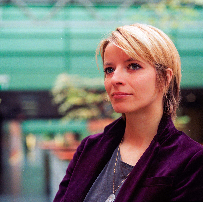
\includegraphics[width=0.9\textwidth]{images/portrait}
    	\end{center}
    	\href{https://www.uwo.ca/philosophy/people/vidotto.html}{Prof. Francesca Vidotto} is a theoretical physicist and philosopher working in the areas of loop quantum gravity, foundations of physics and aspects of epistemology, among others. She completed her undergraduate at the University of Padova and her PhD from the University of Pavia and Aix-Marseille Université. She went on to hold postdoctoral positions at the University of Grenoble, Nijmegen and Bilbao. She is the recipient of the Rubicon and the Veni fellowship by the Netherlands Organization for Scientific Research. Since 2019, she is a professor of Physics \& Astronomy and Philosophy at the University of Western Ontario and she holds the Canada research chai in Foundations of Physics. She is also a core member of the Rotman Institute of Philosophy.
    \end{block}


%%%%%%%%%%%%%%%%%%%%%%%%%%%%%%%%%%%%%%%%%%%%%%%%%%%%%
%            BLOCK: RESEARCH INTERESTS              %
%%%%%%%%%%%%%%%%%%%%%%%%%%%%%%%%%%%%%%%%%%%%%%%%%%%%%
    \begin{block}{Research Interests}
        Prof. Vidotto's research explores the quantum aspects of the gravitational field. This involves a reflection on the nature of space and time, as well as the foundations of quantum mechanics. In particular, she is interested in the structural, relational, and perspectival aspects in those theories. I am considering the contribution of different epistemologies, in particular feminist epistemology, in order to understand the relational ontology that emerges from current theoretical physics. 
        \begin{center}
	    	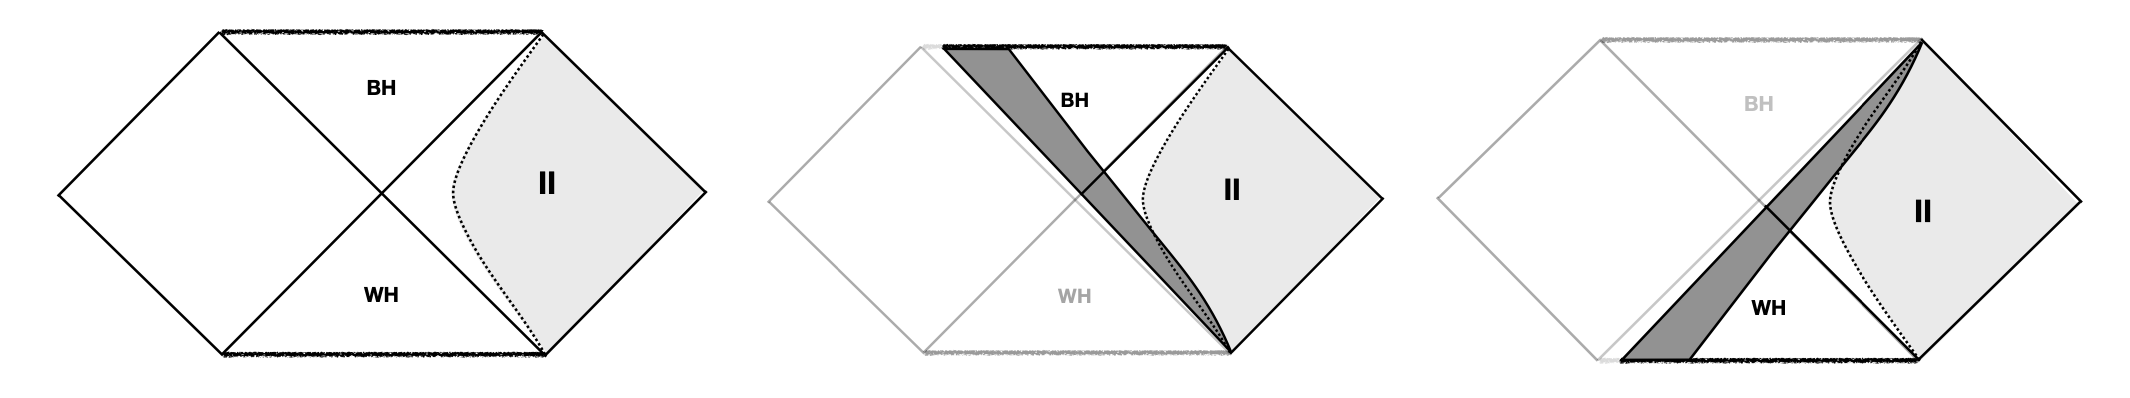
\includegraphics[width=0.9\textwidth]{images/research}    		

    	\textit{Various Spacetime diagrams. \cite{rovelliWhiteholeDarkMatter2018}} 
    	\end{center}

    \end{block}
\end{column}
\begin{column}{0.55\textwidth - 1cm}


%%%%%%%%%%%%%%%%%%%%%%%%%%%%%%%%%%%%%%%%%%%%%%%%%%%%%
%                 BLOCK: ABSTRACT                   %
%%%%%%%%%%%%%%%%%%%%%%%%%%%%%%%%%%%%%%%%%%%%%%%%%%%%%
    \begin{block}{Talk Abstract}
    	While well-known mathematical descriptions of black holes consider them as eternal objects, physical black holes are dynamical objects with a finite life: they form, they evolve, and eventually they exhaust themselves. The end of black holes is the least understood aspect of their evolution. In this colloquium I discuss the ongoing research on this. I focus on two phases of black hole like, that can follow (or even supersede) the Hawking evaporation: a short white-hole phase and a long remnant phase. I discuss some recent progress concerning the black-to-white transition, the main characteristic of the remnant phase, and how remnants can play a role in cosmology as a (dark) matter component.
    \end{block}


%%%%%%%%%%%%%%%%%%%%%%%%%%%%%%%%%%%%%%%%%%%%%%%%%%%%%
%                BLOCK: BACKGROUND                  %
%%%%%%%%%%%%%%%%%%%%%%%%%%%%%%%%%%%%%%%%%%%%%%%%%%%%%
    \begin{block}{Brief Background}
    	A black-hole forms in the collapse of some matter and is accompanied by the formation of a horizon. In the physical world, this horizon is not a strict event horizon but rather a dynamical horizon with a finite lifetime and can be modeled as a trapping surface. The collapse of the black hole may continue beyond the surface until it reaches a maximum contraction at which point it becomes a Planck star. At this scale, factors like effective quantum pressure becomes relevant and leads to an expansion and subsequently the creation of an anti-trapping surface, known as the white-hole. This passage from a contracting to an expanding scenario is called the bounce. Thus, two classical solutions, the white-hole and the black-hole, of the Einstein equation are related by a quantum regime which can be understood by quantum tunnelling. Akin to examples of nuclear decay, we can understand the black-hole to white-hole tunnelling as a decay and ask questions about lifetime and time-scale of events. \cite{rovelliSmallBlackWhite2018}     
    	%\cite{longLocalAxonalConduction2020} 
        \begin{center}
		   	
\includegraphics[width=0.45\textwidth]{images/background}    		

    	\textit{The full life of a black-white hole.\cite{rovelliWhiteholeDarkMatter2018} } 
    	\end{center}
    \end{block}


%%%%%%%%%%%%%%%%%%%%%%%%%%%%%%%%%%%%%%%%%%%%%%%%%%%%%
%                 BLOCK: REFERENCES                 %
%%%%%%%%%%%%%%%%%%%%%%%%%%%%%%%%%%%%%%%%%%%%%%%%%%%%%
    \begin{block}{References}
    \nocite{*}
        \bibliographystyle{aipnum4-1}
%        \bibliographystyle{iopart-num}
		\bibliography{references}
    \end{block}

\end{column}
\end{columns}


%%%%%%%%%%%%%%%%%%%%%%%%%%%%%%%%%%%%%%%%%%%%%%%%%%%%%
%                    FOOTER TEXT                    %
%%%%%%%%%%%%%%%%%%%%%%%%%%%%%%%%%%%%%%%%%%%%%%%%%%%%%
\begin{textblock}{0.5}(0.18, 0.94)
    \color{white}
    \sffamily
    \textbf{Eberly College of Science}
    \\
    Department of Physics
\end{textblock}


%%%%%%%%%%%%%%%%%%%%%%%%%%%%%%%%%%%%%%%%%%%%%%%%%%%%%
%                   END TEMPLATE                    %
%%%%%%%%%%%%%%%%%%%%%%%%%%%%%%%%%%%%%%%%%%%%%%%%%%%%%
\end{frame}
\end{document}
